\documentclass[12pt]{article}
\usepackage{lecture}
\usepackage{graphicx}
\usepackage{epstopdf}
\usepackage{html}
\usepackage{url}

\newcommand{\copyrightYears}{2019-2023}

\title{Genomic prediction: a brief overview}

\begin{document}

\maketitle

\thispagestyle{first}

\section*{Introduction}

Let's review the basic approach we use in genome-wide association
mapping.

\begin{itemize}

\item We measure both the phenotype, $y_i$, of individual $i$ and its
  genotype at a large number of loci, where $x_{ij}$ is the
  individual's genotype at locus $j$.

\item We regress phenotype on genotype one locus at a time, using a
  random effect to correct for phenotypic similarities that reflect
  relatedness rather than similarity in genotype. 
\[
y_i^{(k)} = x_{ij}\beta_j + \phi^{(k)} + \epsilon_i \quad .
\]

\end{itemize}

Keep in mind this is a highly idealized schematic of how GWAS analyses
are actually done.\footnote{Remember, also, that in analyses of human
  disease, a case-control approach is often used rather than the
  regression approach I've been focusing on.} If you want to do GWAS
for real, you should take a look at
GEMMA~(\url{http://www.xzlab.org/software.html})\index{GEMMA} or
TASSEL~(\url{https://www.maizegenetics.net/tassel}).\index{TASSEL} One
important way in which what I've presented is a simplification is that
in a real GWAS analysis, you'd estimate the effects of every locus
simultaneously, which raises an interesting problem.

In a typical GWAS analysis\footnote{In humans at least}, you will have
measured the phenotype of a few thousand individuals, but you will
have genotyped those individuals at several hundred thousand
loci. Lango Allen et al.~\cite{LangoAllen-etal-2010}, for example,
report results from a large analysis of height variation in humans,
183,727 individuals genotyped at 2,834,208 loci. What's the problem
here?

There are more predictors~(loci) than observations~(individual
phenotypes). If you remember some basic algebra, you'll remember that
you can't solve a set of linear equations unless you have the same
number of equations as unknowns. For example, you can't solve a set of
three equations that has five unknowns. There's a similar phenomenon
in statistics when we're fitting a linear regression. In statistics we
don't ``solve'' an equation. We find the best fit in a regression, and
we can do so in a reasonable way so long as the number of observations
exceeds the number of variables included in our regression. To put a
little mathematical notation to it, if $n$ is the number of
observations and $p$ is the number of regression parameters we hope to
estimate, life is good (meaning that we can estimate the regression
parameters) so long as $n > p$.\footnote{And the more that $n$ exceeds
  $p$ the better, the more accurate our estimates of the regression
  parameters will be.} The typical situation we encounter in GWAS is
that $n < p$, which means we have to be really sneaky. Essentially
what we do is that we find a way for the data to tell us that a lot of
the parameters don't matter and we fit a regression only to the ones
that do, {\it and\/} we set things up so that the remaining number of
parameters is less than $n$. If that all sounds a little hoky, trust
me it isn't. There are good ways to do it and good statistical
justification for doing it\footnote{And biological justification for
  doing it in GWAS.}, but the mathematics behind it gets pretty hairy,
which is why you want to use GEMMA or TASSEL for a real GWAS. We'll
ignore this part of the challenge associated with GWAS and focus on
another one: complex traits often are influenced by a very large
nubmer of loci. That is, after all, why we started studying
quantitative genetics in the first place.

\section*{Genetics of complex traits}

Let's return to that Lango Allen et al.~\cite{LangoAllen-etal-2010}
GWAS on height in humans. They identified at least 180 loci associated
with differences in height. Moreover, many of the variants are closely
associated with genes that are part of previously identified pathways,
e.g., Hedgehog signaling,\footnote{``The Hedgehog signaling pathway is
  a signaling pathway that transmits information to embryonic cells
  required for proper cell differentiation.''
  \url{https://en.wikipedia.org/wiki/Hedgehog_signaling_pathway},
  accessed 14 August 2021.} or that were previously identified as
being involved in skeletal growth defects. A more recent study by Wood
et al.~\cite{Wood-etal-2014} synthesized results from 79 studies
involving 253,288 individuals and identified 697 variants that were
clustered into 423 loci affecting differences in height.\footnote{It's
  worth noting that even this is likely to be an underestimate of the
  number of loci associated with height variation in humans because
  all of the individuals included in the analysis were of European
  ancestry.} Think about what that means. If you know my genotype at
only one of those 697 variants, you know next to nothing about how
tall I am~(Figure \ref{fig:GWAS-small-effect}). But what if you knew
my genotype for all of those variants? Then you should be able to do
better.\index{Genome-wide association study!human height}

\begin{figure}
  \begin{center}
    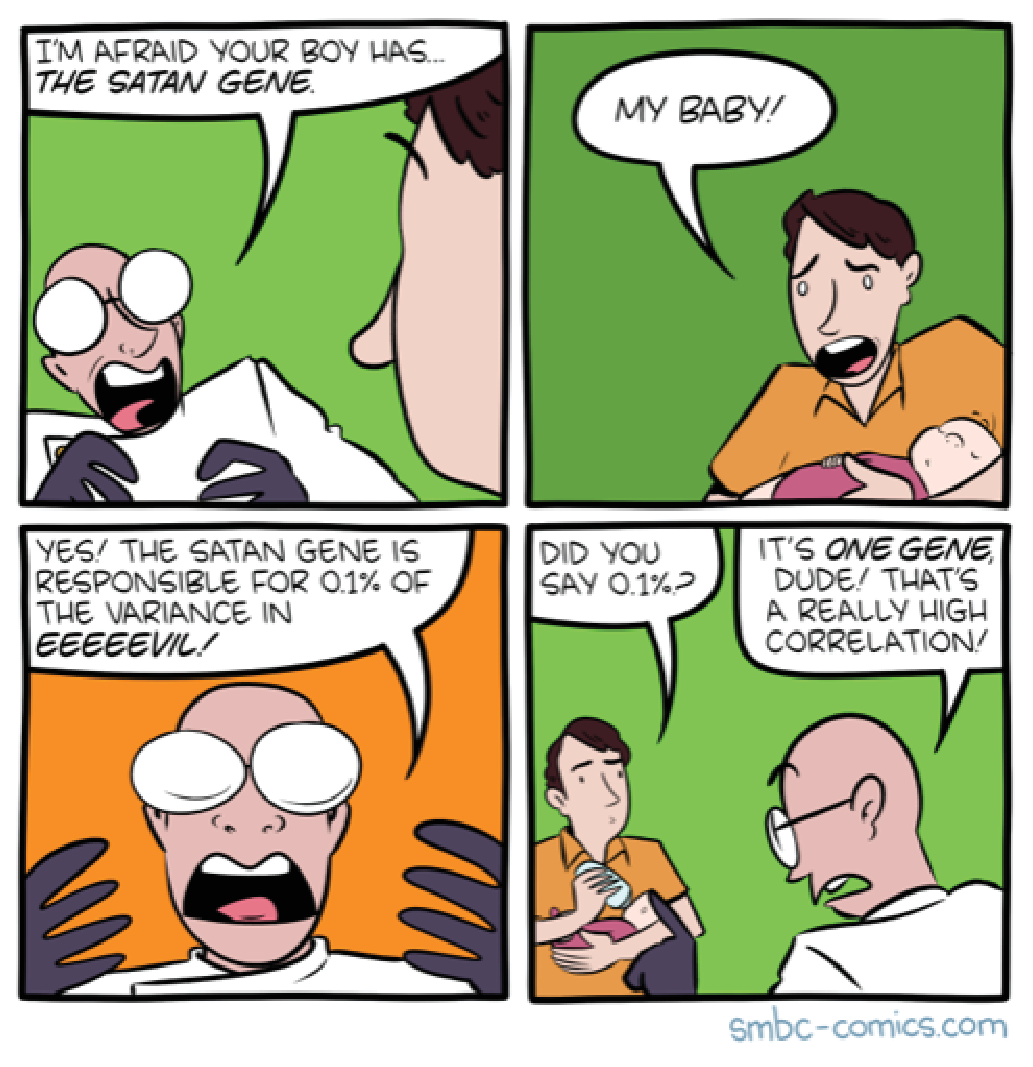
\includegraphics[height=6cm]{GWAS-small-effect.eps}
  \end{center}
  \caption{If a trait is influenced by a large number of genes, the
    effect of any one of them is likely to be very small.}\label{fig:GWAS-small-effect}
\end{figure}

The basic idea is fairly simple. When you do a full GWAS and estimate
the effects at every locus simultaneously, you are essentially
performing a multiple regression of phenotype on all of the loci
you've scored simultaenously instead of looking at them one at a
time. In equation-speak,
\[
y_i^{(k)} = \sum_j x_{ij}\beta_j + \phi^{(k)} + \epsilon_i \quad .
\]
Now think a bit more about what that equation means. The $\phi^{(k)}$
and $\epsilon_i$ terms represent random variation, in the first case
variation that is correlated among individuals depending on how
closely related they are and in the second case variation that is
purely random. The term $\sum_j x_{ij}\beta_j$ reflects systematic
effects associated with the genotype of individual $i$. In other
words, if we know individual $i$'s genotype, i.e., if we know $x_{ij}$
we can predict what phenotype it will have, namely
$\mu_i = \sum_j x_{ij}\beta_j$. Although we know there will be
uncertainty associated with this prediction, $\mu_i$ is our best guess
of the phenotype for that individual, i.e., our genomic prediction or
polygenic score. In the case of height in human beings, it turns out
that the loci identified in Wood et al.~\cite{Wood-etal-2014} account
for about 16 percent of variation in height.\footnote{In Europe the
  heritability of height at age 20 is about 80
  percent~\cite{Jelenkovic-etal-2016}.}\index{genomic predictioon}
\index{polygenic score} If we don't have too many groups, we could
refine our estimate a bit further by adding in the group-specific
estimate, $\phi^{(k)}$. Of course when we do so, our prediction is no
longer a {\it genomic\/} predictiion, {\it per se}. It's a genomic
prediction enhanced by non-genetic group information.

\subsection*{A toy example}

To make all of this more concrete, we'll explore a toy example using
the highly simplified one locus at a time approach to GWAS with a
highly simplified example of the multiple regression approach to
GWAS. You'll find an {\tt R} notebook that implements all of these
analyses at
\url{http://darwin.eeb.uconn.edu/eeb348-notes/Exploring-genomic-prediction.nb.html}. I
encourage you to download the notebook as you follow along. You will
find it especially useful if you try some different scenarios by
changing {\tt nloci} and {\tt effect} when you generate the data that
you later analyze locus by locus or with genomic prediction. Here's
what the code as written does:

\begin{itemize}

\item Generate a random dataset with 100 individuals and 20 loci, 5 of
  which influence the phenotype. The simulation is structured so that
  allele frequencies are correlated across the loci. The effect of one
  ``1'' allele at locus 1 is 1, at locus 2 -1, at locus 3 0.5, at
  locus 4 -0.5, and at locus 5 0.25. The standard deviation of the
  phenotype around the predicted mean is 0.2.

\item Run the locus-by-locus regression for each locus and store the
  results (mean and 95\% credible interval) in {\tt results}. {\tt
    results} is sorted in by the magnitude of the posterior mean, so
  that loci with the largest estimated effect occur at the top and
  loci with the smallest effect occur at the bottom.

\item Run the multiple regression and store the results in {\tt
    results\_gp}.  
    
\end{itemize}

If you look at the code, you'll see that I use {\tt stan\_lm()} rather
than using {\tt brm}. That's because I simulate the data without
family structure, so there's no need to include the family random
effect.

Table~\ref{table:single} shows results of the locus by locus analysis.

\begin{table}
  \centering
\begin{tabular}{rrrr}
  \hline
 & mean & 2.5\% & 97.5\% \\ 
  \hline
locus\_2 & -1.013 & -1.184 & -0.800 \\ 
locus\_1 & 0.979 & 0.687 & 1.270 \\ 
locus\_4 & -0.743 & -1.086 & -0.406 \\ 
locus\_5 & 0.462 & 0.027 & 0.906 \\ 
locus\_3 & 0.390 & 0.039 & 0.742 \\ 
locus\_20 & -0.382 & -0.857 & 0.081 \\ 
locus\_8 & 0.374 & -0.001 & 0.764 \\ 
locus\_7 & -0.327 & -0.681 & 0.052 \\ 
locus\_12 & 0.271 & -0.144 & 0.671 \\ 
locus\_6 & 0.235 & -0.220 & 0.691 \\
locus\_11 & 0.191 & -0.391 & 0.784 \\ 
locus\_13 & -0.173 & -0.557 & 0.209 \\ 
locus\_10 & -0.113 & -0.490 & 0.258 \\ 
locus\_19 & -0.106 & -0.437 & 0.239 \\ 
locus\_14 & -0.093 & -0.555 & 0.347 \\ 
locus\_15 & 0.075 & -0.280 & 0.421 \\ 
locus\_18 & -0.061 & -0.434 & 0.308 \\ 
locus\_17 & 0.050 & -0.362 & 0.458 \\ 
locus\_16 & -0.009 & -0.350 & 0.331 \\ 
locus\_9 & 0.007 & -0.370 & 0.396 \\
  \hline
\end{tabular}
\caption{Sample results for locus by locus analysis of genetic
  associations}\label{table:single}
\end{table}

For this simulated data set the five loci with the largest estimated
effect are the same five loci for which the simulation specified an
effect, but notice the locus 20 and locus 8 have estimated allelic
effects almost as large as the top five and that the estimate for
locus 8 barely overlaps zero. Given only these results it would be
reasonable to conclude that we have evidence for an effect of locus 20
and locus 8, although the evidence is weak. 

What about the multiple regression approach? First, take a look at the
estimated effects~(Table~\ref{table:multiple}). Not only does this
approach pick out the right loci, the first five, none of the other
loci have particularly large estimated effects. The largest, {\tt
  locus\_17} is only about -0.08. It would take much more extensive
simulation to demonstrate the advantage empirically, but it is clear
from first principles that multiple regression analyses will generally
be more reliable than locus by locus analyses because a multiple
regression analysis takes account of random associations among loci.

\begin{table}
\centering
\begin{tabular}{rrrr}
  \hline
 & mean & 2.5\% & 97.5\% \\ 
  \hline
locus\_1 & 1.039 & 0.898 & 1.175 \\
locus\_2 & -0.971 & -1.120 & -0.820 \\
locus\_3 & 0.586 & 0.441 & 0.724 \\
locus\_4 & -0.521 & -0.667 & -0.369 \\
locus\_5 & 0.353 & 0.153 & 0.538 \\
locus\_17 & -0.082 & -0.254 & 0.028 \\
locus\_13 & 0.062 & -0.037 & 0.208 \\
locus\_7 & -0.058 & -0.205 & 0.038 \\
locus\_10 & 0.047 & -0.047 & 0.196 \\
locus\_9 & -0.030 & -0.166 & 0.062 \\
locus\_14 & 0.020 & -0.089 & 0.166 \\
locus\_8 & 0.018 & -0.078 & 0.149 \\
locus\_18 & 0.016 & -0.076 & 0.128 \\
locus\_16 & 0.014 & -0.076 & 0.123 \\
locus\_20 & 0.011 & -0.100 & 0.142 \\
locus\_6 & -0.009 & -0.136 & 0.107 \\
locus\_11 & -0.008 & -0.159 & 0.121 \\
locus\_12 & 0.008 & -0.097 & 0.123 \\
locus\_15 & 0.003 & -0.090 & 0.103 \\
locus\_19 & 0.000 & -0.091 & 0.094 \\
  \hline
\end{tabular}
\caption{Results from multiple regression analysis of simulated
  data.}\label{table:multiple} 
\end{table}

\section*{Comparing the results}

Let's see what other differences we find when we compare the two
approaches more directly. First, let's look at the estimated allelic
effects themselves~(Figure~\ref{fig:gwas-vs-gp}). As you can see, they
are broadly similar, but if you look closely, they are most similar
when the estimated allelic effects are small.

\begin{figure}
  \begin{center}
    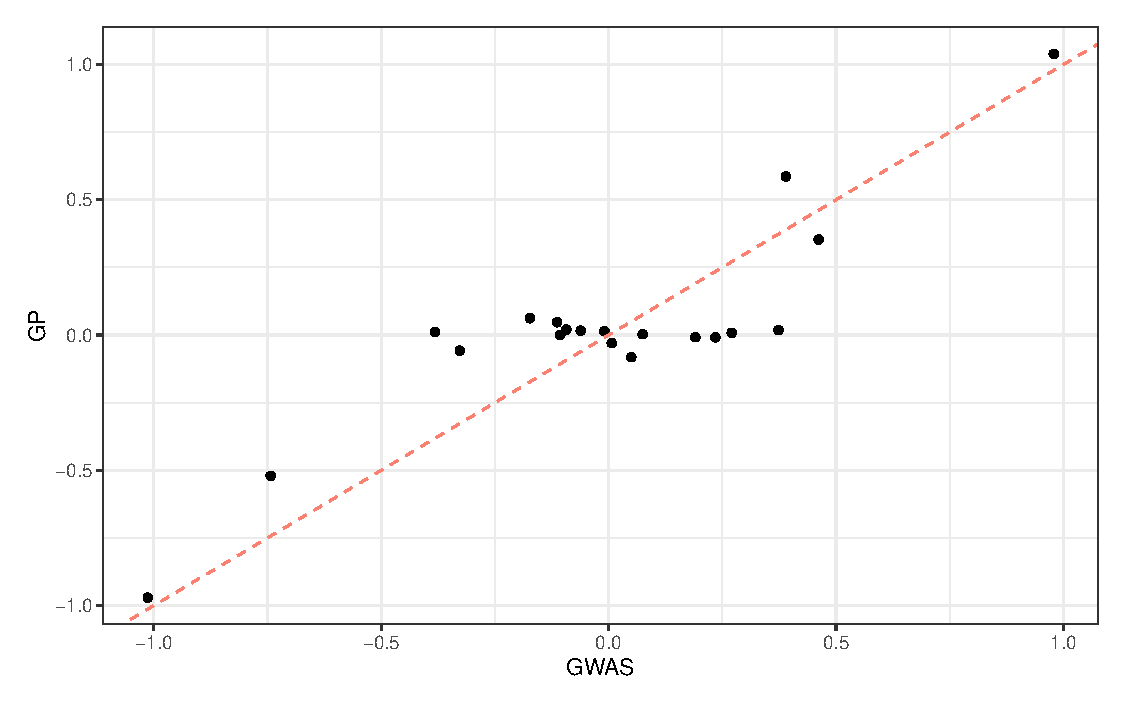
\includegraphics[width=10cm]{gwas-vs-gp.eps}
  \end{center}
  \caption{Estimated allelic effects from locus-by-locus GWAS (x-axis)
    and genomic prediction (y-axis).}\label{fig:gwas-vs-gp}
\end{figure}

More interesting than whether the estimated allelic effects are
similar is whether the predicted phenotypes are similar to the
observed phenotypes~(Figure~ref{fig:gwas-obs-vs-predicted}). As you
can see, in this simple simulated data set both approaches work
reasonably well, even though the estimated allelic effects are rather
different. As expected, though, the multiple regression approach has
less error than the locus-by-locus approach, an $R^2$ of 11.1 vs.\
14.2. 

\begin{figure}
  \begin{center}
    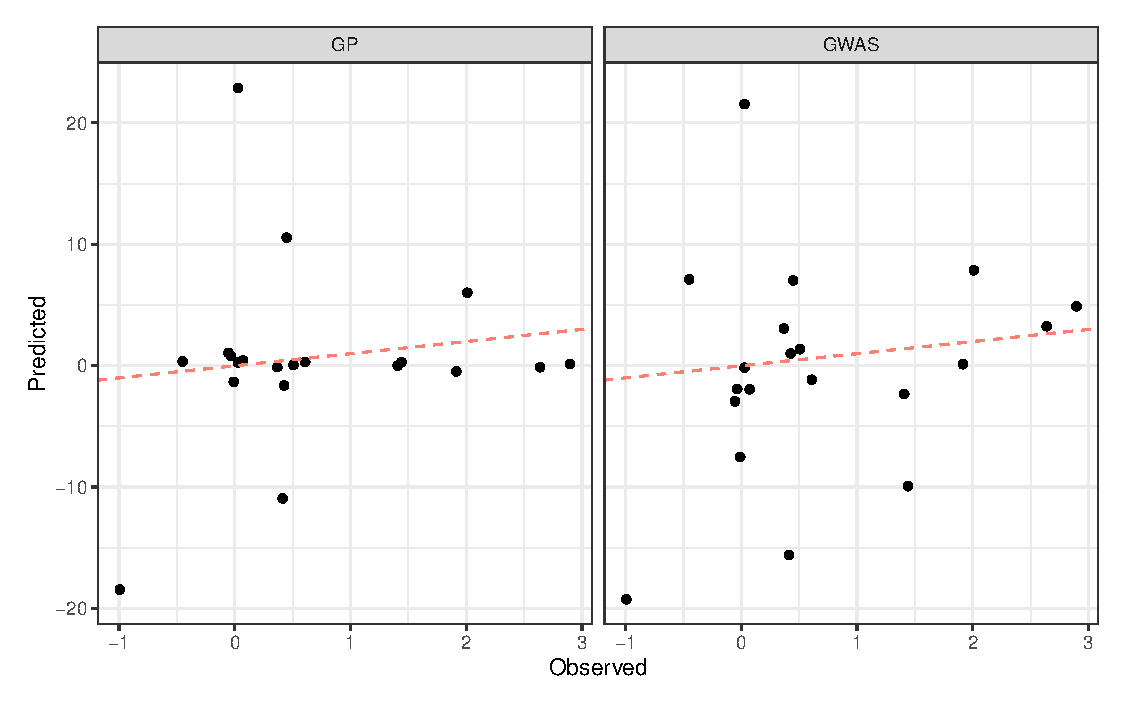
\includegraphics[width=10cm]{gwas-obs-vs-predicted.eps}
  \end{center}
  \caption{Predicted phenotypes {\it versus\/} observed phenotypes for
    locus-by-locus GWAS and genomic prediction.}\label{fig:gwas-obs-vs-predicted}
\end{figure}

\section*{Some caveats about genomic prediction}

In the early 2010s, Turchin and
colleagues~\cite{Turchin-etal-2012}\footnote{{\it Michael\/} Turchin,
  not {\it Peter\/} Turchin of UConn's EEB department.} studied the
association between variation at SNP loci and height in humans. They
showed that both individual alleles known to be associated with
increased height and in genome-wide analysis are elevated in northern
European populations compared to populations from southern
Europe. They argued that these differences were consistent with weak
selection at each of the loci~($s \approx [10^{-3}, 10^{-5}]$) rather
than genetic drift alone.

\subsection*{Allele frequency comparisons}

Turchin et al.\ used allele frequency estimates from the Myocardial
Infarction Genetics consortium~(MIGen)~\cite{MIGen-2009} and the
Population Reference Sample~(POPRES)~\cite{Nelson-etal-2008}. For the MIGen
analysis, they compared allele frequencies in 257 US individuals of
northern European ancestry with those in 254 Spanish individuals at
loci that are known to be associated with height based on GWAS
analysis\footnote{See Turchin et al. for details.} and found
differences greater than those expected based on 10,000 SNPs drawn at
random and matched to allele frequencies at the target loci in each
population. They performed a similar analysis with the POPRES sample
and found similar results.

Turchin et al. were aware that the association could be spurious if
ancestry was not fully accounted for in these analyses, so they also
used data collected by the Genetic Investigation of ANthropometric
Traits consortium (GIANT)~\cite{LangoAllen-etal-2010}.\footnote{This
  includes the GWAS on height that I mentioned in the last lecture.}
They noted that ``control'' SNPs used in the preceding analysis,
i.e., the 10,000 SNPs drawn at random from the genome, with a tendency
to increase height in the GIANT analysis also tended to be more
frequent in the northern European sample.

They compared the magnitude of the observed differences at the most
strongly associated 1400 SNPs with what would be expected if they were
due entirely to drift and what would be expected if they were due to a
combination of drift and selection. A likelihood-ratio test of the
drift alone model {\it versus\/} the drift-selection model provided
strong support for the drift-model.

\section*{Second thoughts}

\subsection*{Within sample stratification}\index{genomic prediction!sample stratification}

This all seems very promising, but a word of caution is in order. Berg
et al.~\cite{Berg-etal-2018} re-examined these claims using new data
available from the UK
Biobank~(\url{https://www.bdi.ox.ac.uk/research/uk-biobank}), which
includes a host of information on individual phenotypes as well as
genome-wide genotypes for the 500,000 individuals included in the
sample.\footnote{Although all of the samples are from the UK, one of
  the data sets Berg et al.~\cite{Berg-etal-2018} studied included
  individuals of European, but non-UK, ancestry.} They failed to
detect evidence of a cline in polygenic scores in their
analysis~(Figure~\ref{fig:UK-biobank}).

\begin{figure}
  \begin{center}
    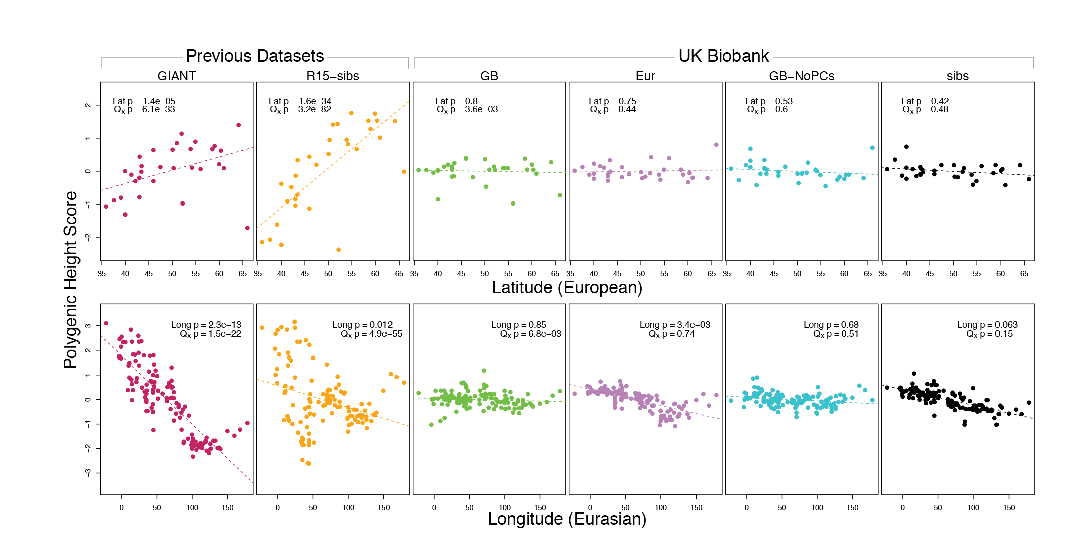
\includegraphics[width=\textwidth]{UK-biobank.eps}
  \end{center}
  \caption{Polygenic score as a function of latitude and longitude for
    several different GWAS data sets. Each vertical column corresponds
  to a different data source. Notice that all of the UK Biobank
  samples fail to show either a latitudinal or a longitudinal cline in
  polygenic height score~(from \cite{Berg-etal-2018}).}\label{fig:UK-biobank} 
\end{figure}

In thinking about this result, it's important to understand that Berg
et al.~\cite{Berg-etal-2018} did something a bit different from what
we did, but it's exactly what you'd want to do if polygenic scores
worked. They estimated polygenic scores from each of the data sets
identified in the figure. Then they used those scores to estimate
polygenic scores for a new set of samples derived from the 1000
Genomes and Human Origins projects.\footnote{See Berg et
  al.~\cite{Berg-etal-2018} for details.} Since they did the same
thing with all of the data sets, this difference from what we did
doesn't account for the differences among data sets. As Berg et
al. dug more deeply into the data, they concluded that all of the data
sets ``primarily capture real signals of association with height'' but
that the GIANT and R-15 sibs data sets, the ones that show the
latitudinal (and longitudinal in the case of GIANT) associations do so
because the estimated allelic effects in those data sets failed to
fully remove confounding variation along the major geographic axes in
Europe.

The Berg et al. analysis illustrates how difficult it is to remove
confounding factors from GWAS and genomic prediction
analyses. Turchin et al. are highly skilled population geneticists. If
they weren't able to recognize the problem with stratification in the
GIANT consortium data set, all of us should be concerned about
recognizing it in our own. Indeed, I wonder whether the stratification
within GIANT would ever have come to light had Berg et al. not had
additional large data sets at their disposal in which they could try
to replicate the results.

\subsection*{Difficulties extrapolating polygenic scores}

In one way the Berg et al. results are actually encouraging. They
estimated effects in one set of data and used the genomic regressions
estimated from those data to predict polygenic scores in a new data
set pretty successfully. Maybe it's difficult to be sure that the
polygenic scores we estimate are useful for inferring anything about
natural selection on the traits they predict, but if we could be sure
that they allow us to predict phenotypes in populations we haven't
studied yet, they could still be very useful. Can we trust them that
far?

Unfortunately, the answer appears to be ``No.'' Yair and
Coop~\cite{Yair-Coop-2022} recently studied the relationship between
phenotypic stabilizing selection and genetic differentiation in
isolated populations. They showed that even in a very simple model in
which allelic effects at each locus are the same in both populations,
polygenic scores estimated from one population may not perform very
well in the other. Interestingly, as you can see in
Figure~\ref{fig:yair-coop-predictions}, the stronger the selection and
the more strongly allelic differences influence the phenotype, the less
well genomic predictions in one population work in the other.

\begin{figure}
  \begin{center}
    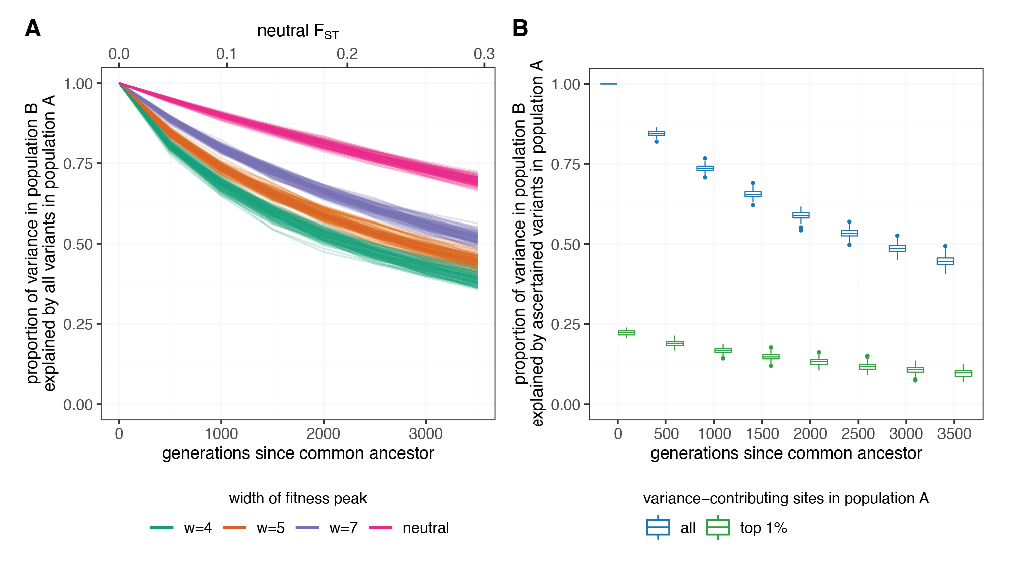
\includegraphics[width=\textwidth]{yair-coop-predictions.eps}
  \end{center}
  \caption{Extrapolations of polygenic scores from one population to
    another decrease in effectiveness the longer populations have been
    separated, even if the trait is subject to uniform stabilizing
    selection.~(from~\cite{Yair-Coop-2021}).}\label{fig:yair-coop-predictions} 
\end{figure}

That seems paradoxical, but interestingly it's not too difficult to
understand if we think about what happens when we combine stabilizing
selection with geographical isolation.\footnote{And the fun thing for
  me about this is that we get to finish out the course by returning
  to a paper I wrote with my first master's student more than 30 years
  ago.} First, let's remind ourselves of a fundamental property of
polygenic variation: Different genotypes can produce the same
phenotype. Figure~\ref{fig:redundancy}, which you've seen before,
illustrates this when three loci influence the trait. While there is
only one genotype that produces the dark red phenotype and only one
that produces the white phenotype, there are four genotypes that
produce the light red phenotype, four that produce the medium dark red
phenotype, and six that produce the medium red phenotype. Goldstein
and Holsinger~\cite{Goldstein-Holsinger-1992} called this phenomenon
{\it genetic redundancy}.\index{genetic redundancy} As you can
imagine, the number of redundant genotypes increases dramatically as
the number of loci involved increases.\footnote{If the allelic effects
  are strictly additive, the number of genotypes corresponding to the
  intermediate phenotype is $2N \choose N$ where $N$ is the number of
  loci. For $N=10$, ${2N \choose N} = 184,756$. For $N=100$, ${2N \choose
  N} = 9.05 \times 10^{58}$.}

\begin{figure}
  \begin{center}
    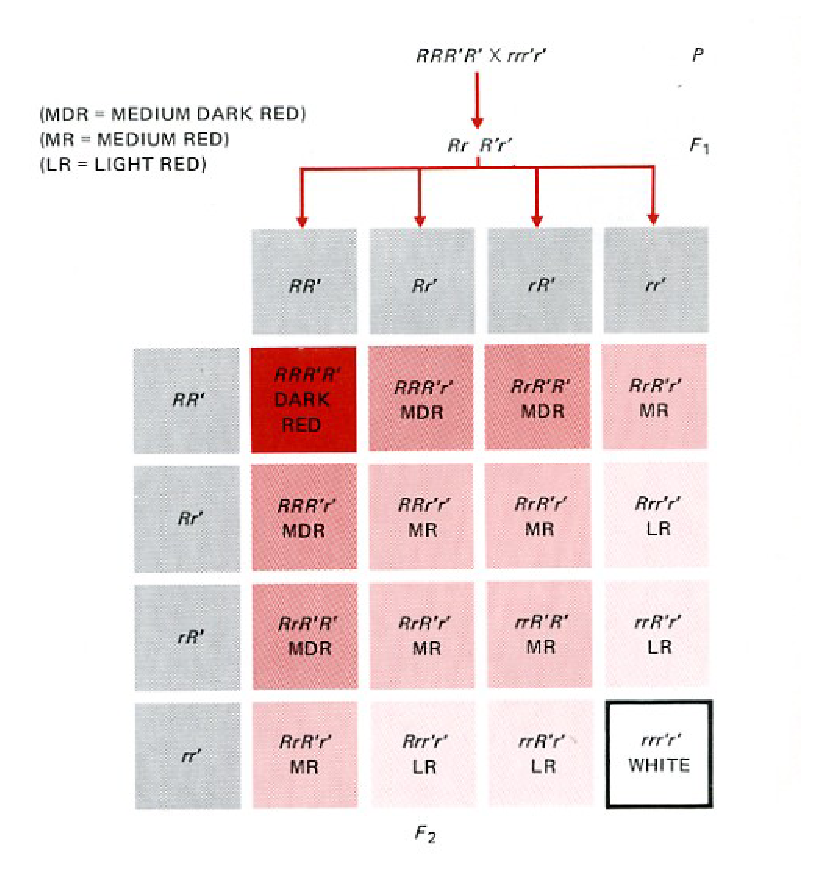
\includegraphics[width=10cm]{Nilsson-Ehle.eps}
  \end{center}
  \caption{Results from one of Nilsson-Ehle's crosses illustrating
    polygenic inheritance of kernel color in wheat~(from {\tt
      http://www.biology-pages.info/Q/QTL.html}, accessed 9 April 2017).}\label{fig:redundancy}
\end{figure}

Why does this redundancy matter? Let's consider what happens when we
impose stabilizing selection on a polygenic trait, where
$$
w(z) = \mbox{exp}\left(\frac{-(z - z_0)^2}{2V_s}\right) \quad ,
$$
where $z_0$ is the intermediate phenotype favored by selection, $z$ is
the phenotype of a particular individual, and $V_s$ is the variance of
the fitness function. If selection is weak ($V_s = 115.2$), then the
relative fitness of a genotype 1 unit away from the optimum is 0.9957
while that of a genotype 8 units away is only 0.7575. If 16 loci
influence the trait, there are 601,080,390 genotypes that produce the
optimum phenotype and have the same fitness. There are another
1,131,445,440 genotypes whose fitness within one percent of the
optimum. Not only are there a lot of different genotypes with roughly
the same fitness, the selection at any one locus is very weak.

Now suppose these genotypes are distributed in a large, continuous
population. Because selection is pretty weak and because mating is
primarily with close neighbors, allele frequency changes at each locus
will be close to what they would be if the loci were neutral. The
result is that the genetic correlation between individuals drops off
rapidly as a function of the distance between
them~(Figure~\ref{fig:isolation-by-distance}). Notice that in the
simulation illustrated individuals separated by more than about 20
distance units are effectively uncorrelated. That means that their
genotypes are essentially random with respect to one another, even
though their phenotypes are similar because of the stabilizing
selection. 

\begin{figure}
\begin{center}
\resizebox{!}{10cm}{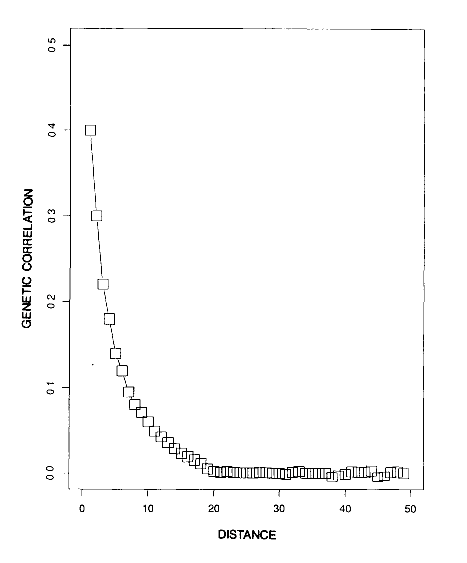
\includegraphics{isolation-by-distance.eps}}
\end{center}
\caption{Isolation by distance with weak
  selection~(from~\cite{Goldstein-Holsinger-1992}).}\label{fig:isolation-by-distance}
\end{figure}

Now think about what that means for polygenic scores. Imagine that we
sampled two ends of a large, continuously distributed population. To
make things concrete, let's imagine that the population is distributed
primarily North-South so that our samples come from a northern
population and a southern one. Now imagine that we've done a GWAS in
the northern population and we want to use the genomic predictions
from that population to predict phenotypes in the southern
population. What's going to happen?

The genotypes in the southern population will be a random sample from
all of the possible genotypes that could produce the same optimal
phenotype (or something close to the optimum) and that sample will be
independent of the sample of genotypes represented in our northern
population. As a result, there are sure to be loci that are useful for
predicting phenotype in the northern population that aren't variable
in the southern population, which will reduce the accuracy of our
genomic prediction. That's precisely what Yair and Coop
show.\footnote{Although their results go much farther than Goldstein
  and Holsinger who did their simulations long before anyone was
  thinking about GWAS, much less genomic prediction and polygenic
  scores.}

In short, it's to be expected that genomic predictions will be useful
only within the population for which they are constructed. They can be
very useful in plant and animal breeding, for example, but any attempt
to use them in other contexts must be alert to the ways in which
extrapolation from one population to another will be problematic.

\bibliography{popgen}
\bibliographystyle{plain}

\ccLicense

\end{document}



